\section{Why adapt?}

In our daily lives, we interact with many different speakers, either truly interactively in conversation or more passively when watching TV, listening to audio or video recordings, or consuming other types of media. Thus, if as listeners, we constantly adapt to all the speakers we encounter and update speaker-specific expectations, we have to keep track of considerable amounts of information. This process clearly incurs some cost, which raises the question what the benefits of adaptation are, and whether the benefits outweigh the cost. I will not be able to answer the latter question since I can neither quantify the 
the cost associated with adaptation nor quantify the utility of adaptation. However, to answer the first question, there exist clear benefits of semantic and pragmatic adaptation, including the following.

First, at the semantic level, listeners will be able to better infer the intended speaker meaning if they know the speaker's mapping between words and world states. For example, if I know that a speaker only uses \emph{some} to refer to quantities greater than 3, I will be better able to narrow down the state of the world after hearing \emph{``I ate some of the cookies''} than I would have been able to if I had assumed that the speaker uses \emph{some} exactly the same way as I do, which for the sake of the example, let's say is to refer to quantities greater than 0. Similarly, differences in speaker and listener meaning become even more striking if my meaning of \emph{some} is narrower than the speaker's \emph{some}: If a speaker uses \emph{some} to refer to a quantity of 4 but my meaning of \emph{some} is limited to quantities greater than 5, I will infer a state of the world that is incompatible with the actual world. \todo{make figure?}.

At the pragmatic level, adaptation can further help listeners to infer the speaker's intended meaning. To see this, note that one of the key assumptions about pragmatic reasoning is that listeners reason about alternative utterances when interpreting a speaker's utterance \cite{Grice1975, Horn1984}. For example, consider the following sentence that gives rise to a scalar implicature.

\begin{exe}
\ex Sue: It might snow tomorrow.
\ex \label{ex:snow-inf} $\rightsquigarrow$  It is not certain that it will snow tomorrow.
\end{exe}

According to Gricean pragmatic theories, listeners assume that a speaker is cooperative and arrive at the inference in (\ref{ex:snow-inf}) through a counterfactual reasoning process: they reason that if Sue had wanted to communicate that it is certain that it will snow tomorrow, Sue would have uttered the more informative statement \textit{It is certain that it will snow tomorrow} (or simply the bare assertion \emph{``It will snow tomorrow''}). Assuming that Sue knew the truth regarding the more informative sentence, it must be that the more informative statement is not true, which leads the listener to conclude (\ref{ex:snow-inf}). 

Accounts of pragmatic reasoning share the implicit assumption that listeners have precise expectations
 about the speaker's language use -- specifically, which utterance alternatives were available to the 
 speaker that they didn't use -- in different situations. Listeners can only draw correct pragmatic 
 inferences if they know what a speaker would have said to communicate alternative world states. 
 In large parts these expectations are guided by the meaning of words. as I illustrated with the cookies example above. 
However, speaker expectations also depend on other factors such as the speaker's preference for
 different lexical items or the set of alternative utterances from which they choose.
 
To illustrate how different beliefs about the meaning of words and utterance preferences can lead to different interpretations, consider the interpretation 
of the uncertainty expression \textit{probably} produced by three different hypothetical speakers. For the sake of this example, 
let us assume the only three expressions that a speaker can choose from are \textit{might}, \textit{probably}, and \textit{almost certainly}.
A listener's beliefs about the three speakers' meanings and preferences are schematically illustrated in Figure~\ref{fig:inference-example}.

% Figure 1: plots/fig-1-implicatures.pdf (2-column figure)
\begin{figure}
\center
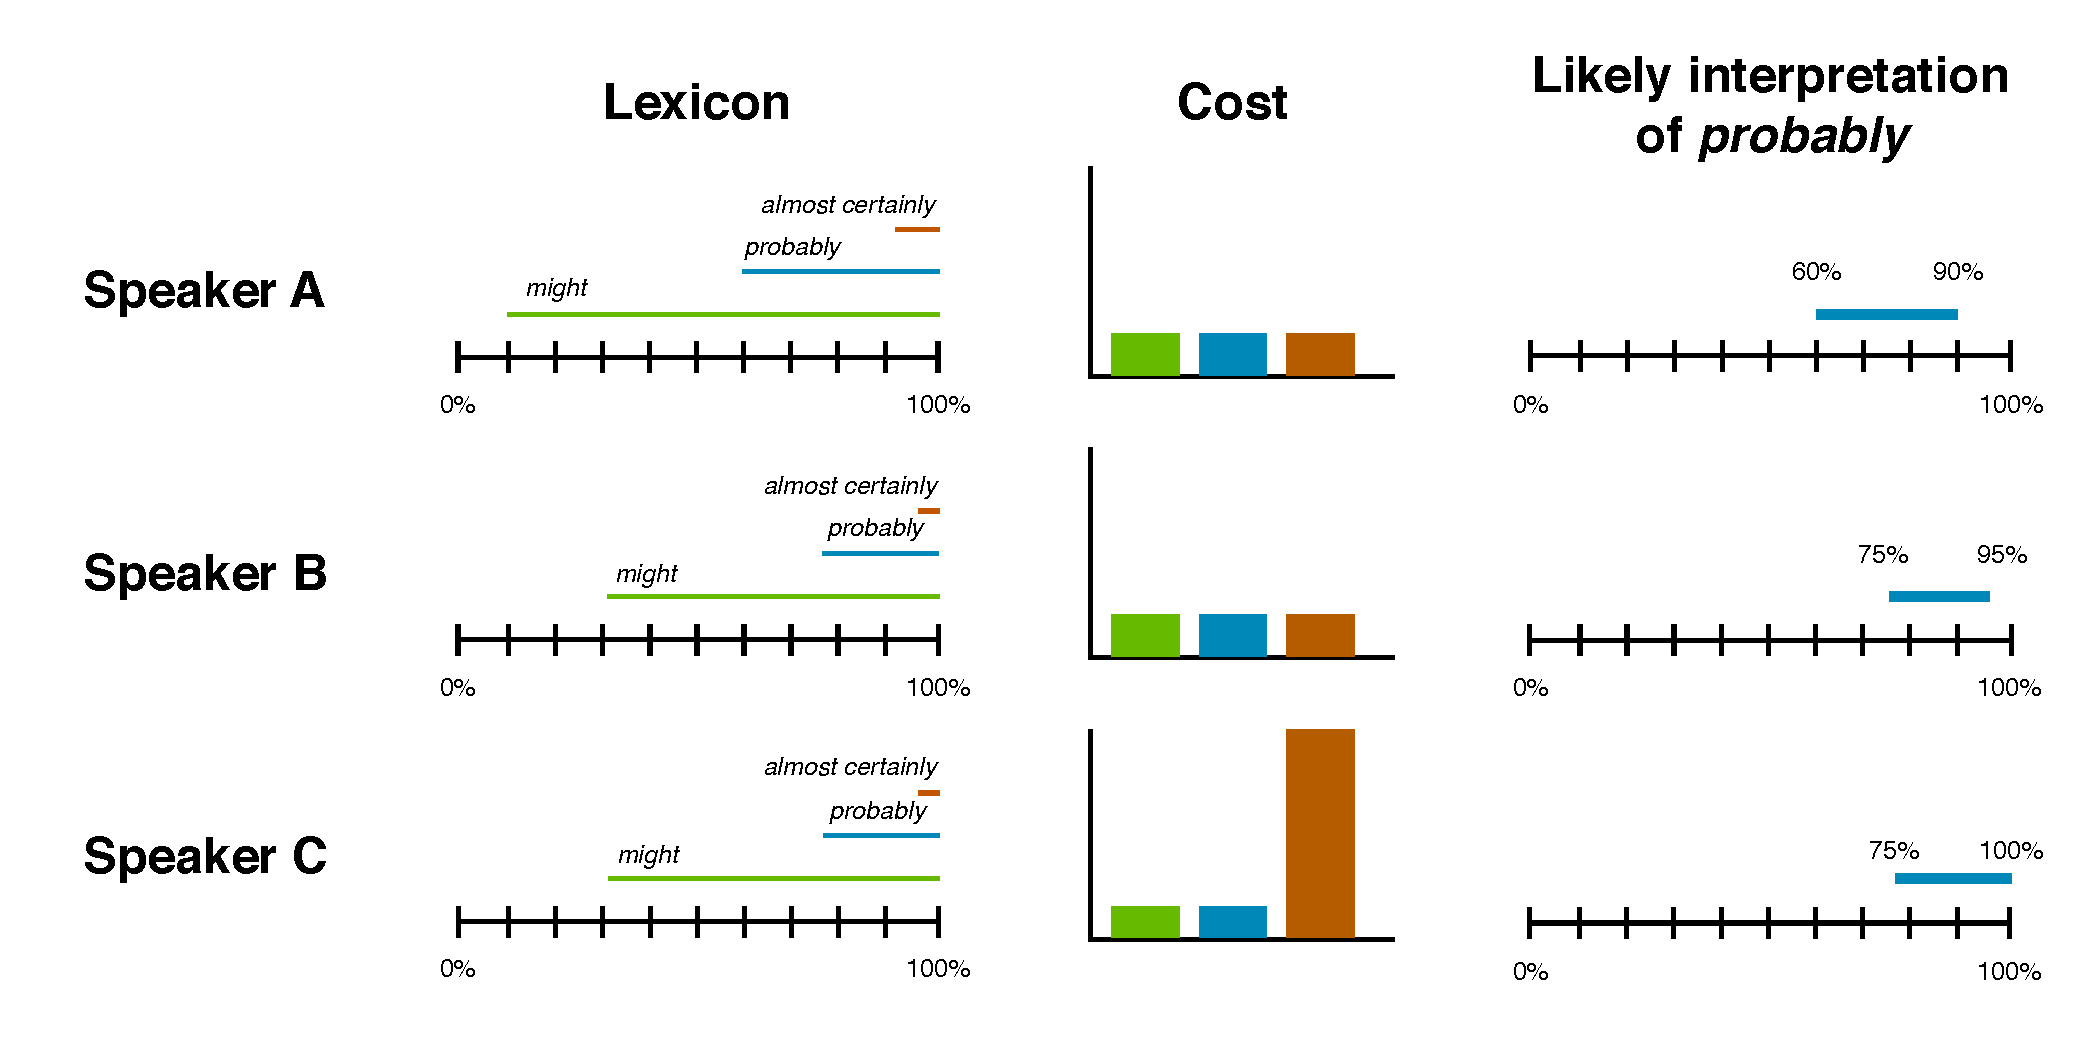
\includegraphics[width=\textwidth]{plots/fig-1-implicatures.pdf}
\caption{Lexica, utterance preferences and likely interpretation of \textit{probably} for three different hypothetical speakers. The region of the probability scale covered by each line in the Lexicon panel indicates the corresponding expression's literal semantics. Height of bars in the Cost panel indicates the speaker's cost (dispreference) for each expression.}
\label{fig:inference-example}
\end{figure}

First, consider speaker {\bf A}, for whom \textit{might} is true if the described event probability (e.g., of snowing) exceeds 10\%, 
\textit{probably} if the event probability exceeds 60\% and \textit{almost certainly}  if the event probability exceeds 90\%.  
If a listener has accurate beliefs about {\bf A}'s mapping between expressions and event probabilities and observes {\bf A} 
produce the sentence \emph{It will probably snow}, they will be likely to infer a probability of snowing between 60 and 90\%. 
As illustrated above, the reasoning follows the schema of a standard scalar implicature \cite{Grice1975, Horn1984}: if  {\bf A} 
had intended to communicate a probability above 90\%, they could have said \emph{It will almost certainly snow}, which would 
have been more informative and equally relevant. Assuming the speaker knows the actual event probability and is cooperative, 
it is therefore likely that the intended probability is not above 90\%.\footnote{Under a standard Gricean view, the negation of the 
stronger alternative is inferred categorically. However, I adopt probabilistic language here in keeping with recent results that scalar 
inferences are more aptly viewed as probabilistic inference under uncertainty \cite{Goodman2013}.} 

Now, consider speaker {\bf B}, for whom \textit{might} is true if the event probability exceeds 30\%, 
\textit{probably} if the event probability exceeds 75\% and \textit{almost certainly}  if the event probability exceeds 95\%. If a listener has
accurate beliefs about {\bf B}'s mappings, they will be likely to infer, via the same reasoning as above, a chance of snow between 75\% and 95\% when they hear {\bf B} produce the same sentence, \textit{It will probably snow}.

Finally, consider speaker {\bf C}. {\bf C} uses the same mapping between expressions and event probabilities as {\bf B}. However, {\bf C} has a strong preference against 
producing \textit{almost certainly}. If a listener has accurate beliefs about {\bf C}'s lexicon and production preferences, 
they will be likely to infer a chance of snow between 75\% and 100\% when they hear {\bf C} produce \textit{It will probably snow} since they will not
consider  \textit{almost certainly} a likely alternative. That is, the scalar inference will be blocked by the additional knowledge of the speaker's production preferences. 

As this example shows, a listener who tracks the variability in these hypothetical speakers' meanings and production preferences 
will draw on average more accurate inferences about the world than a listener who relies on their own meanings and preferences
for interpreting utterances.

The third advantage of adaptation is related to online language processing. The last several decades
in psycholinguistic research produced a lot of evidence that listeners constantly engage in the prediction of 
the upcoming input \cite{e.g.KuperbergJaeger2016}.\footnote{This is more generally true for all perceptual 
processes including vision (see e.g., \cite{Clark2013; Friston2010}).} 
On the one hand, this form of predictive processing makes language comprehension more robust. If due to noise,
a listener is unable to perceive part of the signal, they can often fill in the blanks using their predictive model.
On the other hand, predictive processing makes comprehension more efficient. 
If listeners constantly predict the upcoming signal, the early stages of comprehending an utterance 
reduce to comparing predictions about the upcoming linguistic input to the perceived input and, at these stages, 
listeners only have to process this difference, i.e., the error signal. However, according to such an account,
rapid and accurate processing is only possible if listeners are able to make reliable predictions about the upcoming
input. Accurate predictions in a variable and constantly changing environment, in return, are only possible through
 adaptation which highlights another advantage of constant adaptation.

\section{Defining the scope}

In this dissertation, I investigate the extent of semantic and pragmatic adaptation as well as
the associated cognitive processes. That is, to what extent do listeners learn speaker-specific
meanings of words; to what extent do listeners learn speaker-specific expectations of words,
and to what extent does this speaker-specific knowledge affect interpretations of utterances? 
And what are the cognitive processes that lead to this behavior?

In this enterprise, I focus on uncertainty expressions
such as \emph{might} and \emph{probably}. Thus, all findings will only directly apply to 
adaptation to variable use of uncertainty expressions. However, uncertainty expressions 
belong to the much larger class of context-sensitive expressions -- a class of expressions for 
which it is generally assumed  that their interpretation crucially depends on contextually 
specified parameters which -- as I will show in subsequent chapters --
are also tied to the speaker's identity. Given the extensive research on the parallels between
uncertainty expressions and other context-sensitive expressions such as quantifiers and
gradable adjectives \cite{LassiterBook, SchoellerFranke?}, the results in this dissertation
should therefore also apply to any other types of context-sensitive expressions, and all
the presented models could be easily extended to other classes of expressions. 

\section{Why uncertainty expressions?}
\label{sec:why-uncertainty-expressions}

Uncertainty expressions have several properties that make them a good testing ground for studying semantic and pragmatic
adaptation. First, there is no consistent mapping between uncertainty expressions and event probabilities \cite{e.g., Clark1990,Pepper1974}, 
which suggests that listeners have to rely on additional contextual information (such as speaker identity)
if they want to infer an event probability that a speaker intended to communicate using an uncertainty expression. Second, there is considerable inter-speaker variability 
in the use of these expressions \cite{Wallsten1986} and therefore it is likely that listeners expect different speakers to use these expressions
differently. Lastly, interpreting uncertainty expressions plays an important role in many everyday situations from the banal -- 
such as talking about the weather -- to the serious -- such as communicating about health risks 
\cite{Berry2004, Lipkus2007, Politi2007} or making financial decisions \cite{Doupnik2003}. 
Thus, listeners would benefit from tracking  how a given speaker uses these expressions. 

\section{Structure of this dissertation}

main points of this dissertation:

* comprehension is an extremely flexible process 

* updated interpretations are guided by speaker expectations

* meaning of uncertainty expressions is flexible

* adaptation interacts in complex ways with other contextual factors (e.g., mood)

